\begin{figure}[!t]
  \center {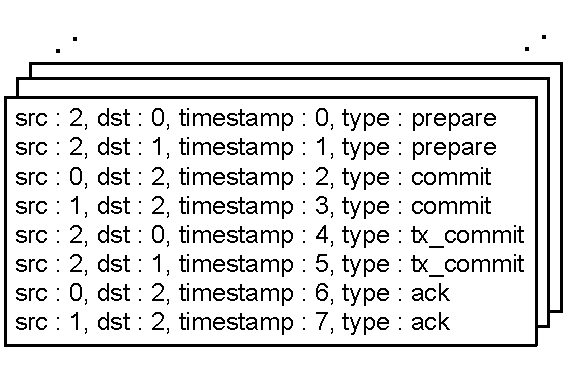
\includegraphics[scale=.6]{img/2pc_trace.pdf}}
  \caption{A partial example trace of a three node run of the
    two-phase commit protocol.}
  \label{fig:2pc_trace}
\end{figure}

\begin{figure}[!t]
  \center {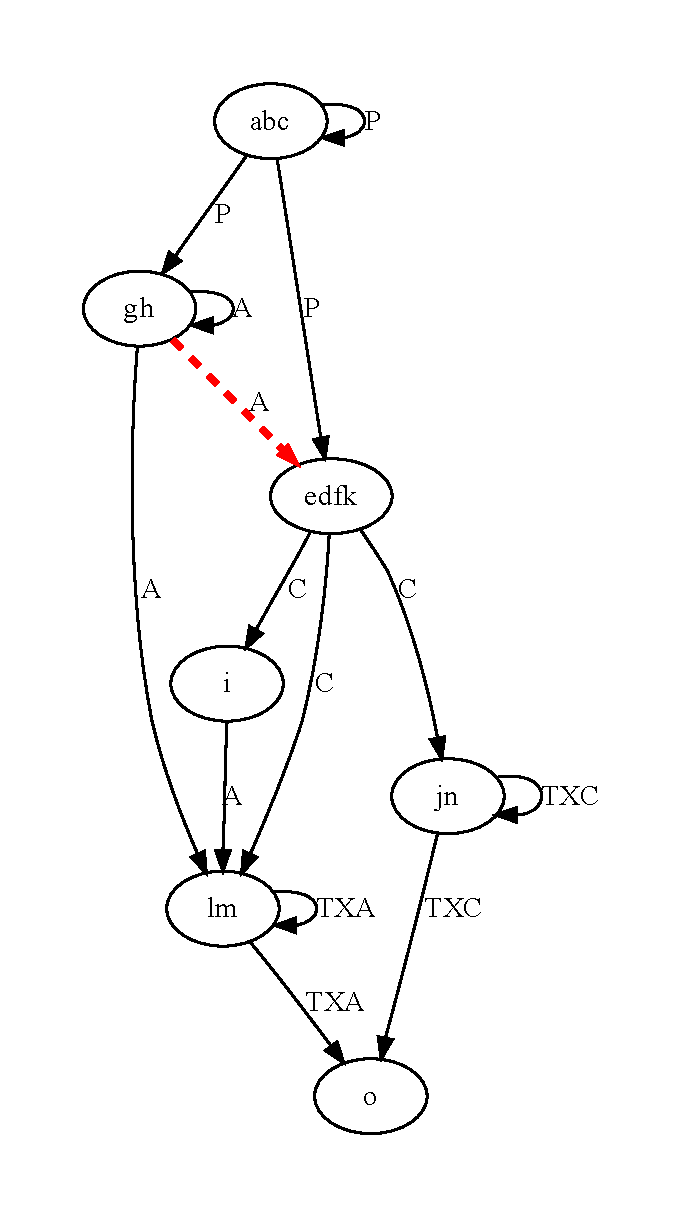
\includegraphics[scale=.6]{img/2pc_k2_inv_bug.pdf}}
  \caption{A Synoptic-generated representation of a buggy two-phase
    commit protocol trace for two nodes, with one transaction
    manager. Transitions represent messages sent/received by a
    replica; states represent abstract system states. States are
    labeled with letters whose combination indicates a particular
    merge of single letter states of the FSM for the non-buggy version
    of the system in Figure~\ref{fig:2pc_k2_inv}. The red dotted edge
    indicates the invalid transition.}
  \label{fig:2pc_k2_inv_bug}
\end{figure}

%%%%%%%%%%%%%%%%%%%%%%%%%%%%%%%%%%%%%%%%%%%%%%%%%%%%%%%%%%%%%%%%%%%%%
\section{Motivation}
%%%%%%%%%%%%%%%%%%%%%%%%%%%%%%%%%%%%%%%%%%%%%%%%%%%%%%%%%%%%%%%%%%%%%

To motivate the problem more concretely we present an example scenario
in which the Synoptic representation of a system trace might help a
developer understand system behavior. We study an atomic commitment
protocol called two-phase commit~\cite{TwoPhaseCommit}, which is
widely used to implement distributed atomic transactions. This
protocol is non-trivial to debug in large systems because it is
inherently concurrent and composed of multiple stages.

% TODO: include structural (e.g. data-oriented) properties

\subsection{A Two-Phase Commit Example}

The two-phase commit protocol must adhere to a number of invariants,
which range over protocol messages -- (P)repare, (C)ommit, (A)bort,
(TXA)bort, (TXC)ommit.  For a system of three nodes (with one node
acting as the transaction manager) Table~\ref{table:twopc_ex_invs}
lists some of the basic invariants.

\begin{table}[!t]
\begin{tabular}{p{3.3cm}p{3.9cm}}
% $\Box(\mathit{TXA}~\rightarrow~\Diamond^-{\mathit{A}})$
  \textbf{Invariants} & \textbf{Explanation}\\
  \hline
  $\Box(\mathit{A}~\rightarrow~\Diamond{\mathit{TXA}})$ & An abort by
  even one replica must prompt an eventual transaction abort.\\
  \hline
  $\Box(\mathit{A}~\rightarrow~\Box{\neg{\mathit{TXC}}})$ & A
  transaction cannot be committed if any replica aborts.\\
  \hline
  $\Box(\mathit{TXC}~\rightarrow~\Box{\neg{\mathit{TXA}}})$
  $\Box(\mathit{TXA}~\rightarrow~\Box{\neg{\mathit{TXC}}})$ & A
  transaction commit and transaction abort are mutually exclusive --
  only one can ever be observed.\\
  \hline
  $|\mathit{C}| + |\mathit{A}| = 2$ & With two-replicas, the
  sum of commit and abort message counts must be two.\\
\end{tabular}

\caption{Some two-phase commit invariants in LTL
  notation. In LTL, $\Box$ and
  $\Diamond$ mean \emph{for all time}, and \emph{eventually}
  respectively.}

\label{table:twopc_ex_invs}
\end{table}

Given a trace that looks like Figure~\ref{fig:2pc_trace}, how can a
developer easily verify whether the invariants in
Table~\ref{table:twopc_ex_invs} hold?  Figure~\ref{fig:2pc_k2_inv_bug}
shows the representation generated by Synoptic for a buggy version of
the system, while Figure~\ref{fig:2pc_k2_inv} (in
section~\ref{sec:evaluation}) shows the representation for a correct
system. It is easy to verify by inspection that all of the above
invariants are maintained in the correct representation. Moreover, the
representation of the buggy system hints at where a problem might lie
-- the second invariant in the Table is violated since in
Figure~\ref{fig:2pc_k2_inv_bug} an A message precedes a TXC message
(the red, dotted edge in the Figure).

Note that the two-phase commit protocol also has non-temporal, or
structural invariants (e.g. the last invariant in
Table~\ref{table:twopc_ex_invs}). Currently Synoptic does not support
such invariants.

% \subsection{A Motivating Example}

% As an example, consider the \texttt{ping-pong} program in which
% $node_1$ periodically sends a ping message to $node_2$ and $node_2$
% immediately replies with a pong message upon receiving the ping. The
% captured trace is a finite sequence of these messages.

% Without considering the message data, the only possible summary of the
% observed behavior is that periodically $node_1$ sends some message to
% $node_2$, and that immediately after $node_2$ sends a message to
% $node_1$. Since message data is excluded from the analysis, it is left
% out of the summary because its informational content is assumed to be
% 0.

% If messages can be compared to one another
% then a simple analysis will reveal an alternating pattern in the
% trace. This pattern can be concisely summarized and must be presented
% to the user to avoid a loss of information from the trace.

% Finally, consider a \texttt{ping-pong} program in which every ping and
% pong message contains a sequence field that are independently
% incremented by 1 before message send by sender. In this case, a simple
% message comparison to find redundancy will reveal that the messages
% are in fact all unique. A more sophisticated approach is
% necessary. For example, the system can infer a relationship between
% the sequence fields of consecutive two ping or consecutive two pong
% messages. This relationship is simply $seq' = seq + 1$. This
% representation captures all the message information content and is a
% concise representation of the message data.

% \subsection{An Uptime Monitoring System}
% \label{subsec:uptime-monitor}

% Consider an uptime monitoring system in which $node_1$ periodically
% sends ping messages to determine whether the other nodes in the system
% are still up. When the ping message is received by $node_i$, the node
% immediately replies with a pong message to $node_1$. When $node_1$
% receives a pong from $node_i$, it sends a status query to $node_i$.
% This is the only pattern of communication in the protocol, and for now
% we assume that ping/pong/status interactions are not interleaved with
% one another. The captured trace of communication is a finite, totally
% ordered sequence of the messages sent and received by $node_1$.

% Considering only message type equivalence, a possible summary of the
% observed behavior is that $node_1$ keeps sending ping messages, and if
% it receives a pong as response, it may send a status message. We would
% like to infer the following \emph{temporal} properties to assure
% ourselves that the system is functioning correctly, at least in so far
% as we can observe it through the generated message traces:

% \begin{itemize}

% \item Pong is only received after sending ping.

% \item Status it only sent after receiving a pong.

% \item The transitive combination of the previous two, i.e.  a status
%   message is only sent after a ping has been sent.

% \item A ping may follow a ping.

% \item A pong need not be followed by a status message.

% \end{itemize}


% \subsection{A MapReduce System}

% Our second example is that of MapReduce~\cite{MapReduce} -- a
% distributed parallel data processing algorithm. It may be desirable to
% use Synoptic to examine a MapReduce system to verify its correctness,
% or to generate proper test cases. We first provide the necessary
% background on how MapReduce works, and then consider the kinds of
% properties that Synoptic might derive from a MapReduce implementation.

% \subsubsection*{Background}

% The system consists of a set $W$ of worker nodes, and a master node
% $M$ (for simplicity we assume that there is just one master node). The
% basic flow of node interactions in the system is as follows:

% \begin{enumerate}

% \item $M$ will send a "start map" control messages to some subset $S
%   \subseteq W$ of the worker nodes. This should begin the "map" phase.

% \item Each node $n_i \in S$ may send 0 or more messages to any nodes
%   in $W$ of the form $\langle k,v \rangle$ corresponding to key-value pairs emitted
%   during the map phase. Call the set of nodes that $n_i$ sent messages
%   to $R_i$.

% \item Each node $n \in S$ will send a "map finished" control message
%   to $M$ to indicate it is done with the "map" phase.

% \item After all "map finished" control messages have been received
%   from all nodes in $S$, $M$ will send a "start reduce" control
%   message to a subset $R \subseteq W$ of worker nodes, exactly equal
%   to the $R = \bigcup_{n_i \in S} R_i$, the set of nodes that were
%   sent key-value pairs during the map phase.

% \item Finally, each node $m_i \in R$, will send a "reduce finished"
%   control message to $M$. After all these messages have been received
%   from all nodes in $R$, the job is complete.

% \end{enumerate}

% \subsubsection*{System Properties}

% The first goal of Synoptic for this system is to model the phases of
% the system as an FSM. Examples of useful features of such an EFSM
% representation are the following:

% \begin{enumerate}

% \item An FSM generated for each worker node should represent a local
%   "map" and "reduce" phase signaled by the sent and received control
%   messages. Specifically this means inferring that no "start reduce"
%   control message was received by the node during the "map" phase, no
%   key-value messages were sent during the "reduce" phase, and all
%   proper control messages were sent and received.

% \item An FSM generated for the master node should represent a global
%   "map" and "reduce" phase. The end of the map phase should be
%   signaled by receiving "map finished" control messages from all
%   nodes in $S$, similarly the end of the reduce phase should be
%   signaled by receiving "reduce finished" control messages from all
%   nodes in $R$.
                                                                                                                                                                                                                                        
% \item A cross-product of the local FSMS generated for every node
%   might reveal that the set $R$ of nodes that were sent "start reduce"
%   control messages from $M$ is the same as the set sent key-value
%   messages during the "map" phase.

% \end{enumerate}

% Additionally, when we bring the contents of messages into the mix, we
% may want to infer further properties. For example:

% The keys sent as part of the key-value messages from mappers to
% reducers satisfy the following constraint: The keyspace $\mathcal{K}$
% is partitioned into disjoint subsets $K_1, K_2, \dots K_j$ by some
% partition function, where $j = |R|$ the number of reducers. The
% partition function is set, and fixed, for the duration of the job and
% may be arbitrary. There exists a map between each $K_i$ and $n_i \in
% R$, call it $g$, such that $g(k) = n_i$ whenever $k \in K_i$, that is
% $g$ assigns the message to a reducer based on key. When a key-value
% message $<k,v>$ is sent from some mapper node, it is sent to the
% reducer assigned by $g(k)$.

% Ideally this may be inferred by Synoptic and would be useful for
% verification or test case generation. This would make sure, for
% example, that a message $<k,v>$ is never sent to some node $n$ such
% that $g(k) \neq n$.

